\chapter{Os metais: reações com os ácidos e corrosão}\label{ch:g9:metals-acids-corrosion}

Num porto, o casco de aço de um velho barco de pesca está riscado de
\omterm{def:g9:metals-acids-corrosion:corrosion}{ferrugem} alaranjada. No cais, um portão revestido de zinco está há
trinta anos na chuva e continua com um brilho cinza fosco. Num museu, um
anel de ouro enterrado durante três mil anos brilha como no dia em que
foi feito. Os metais não enfrentam o mundo todos do mesmo jeito: alguns
são atacados pela água, pelo \omterm{def:g4:air-a-mixture-of-gases:air}{ar} e pelos ácidos, outros quase nada.

\begin{recall}
Os \omterm{def:g9:ions:ion}{íons} são \omterm{def:g7:atoms-and-molecules:atom}{átomos} com carga; os metais dão \omterm{def:g9:ions:ion}{cátions} como \ce{Fe^{2+}},
\ce{Zn^{2+}}, \ce{Al^{3+}}, identificados por testes de \omterm{def:g9:ions:precipitate}{precipitação}
(\cref{ch:g9:ions}). Uma \omterm{def:g9:acids-bases-ph:acidic}{solução ácida} contém muitos \omterm{def:g9:ions:ion}{íons} \ce{H+(aq)}
(\cref{ch:g9:acids-bases-ph}). O hidrogênio \omterm{def:g4:what-a-fire-needs:burning}{queima} com um estalo agudo na
boca de um tubo de ensaio (\cref{ch:g7:identifying-substances}).
\end{recall}

\begin{omfigure}
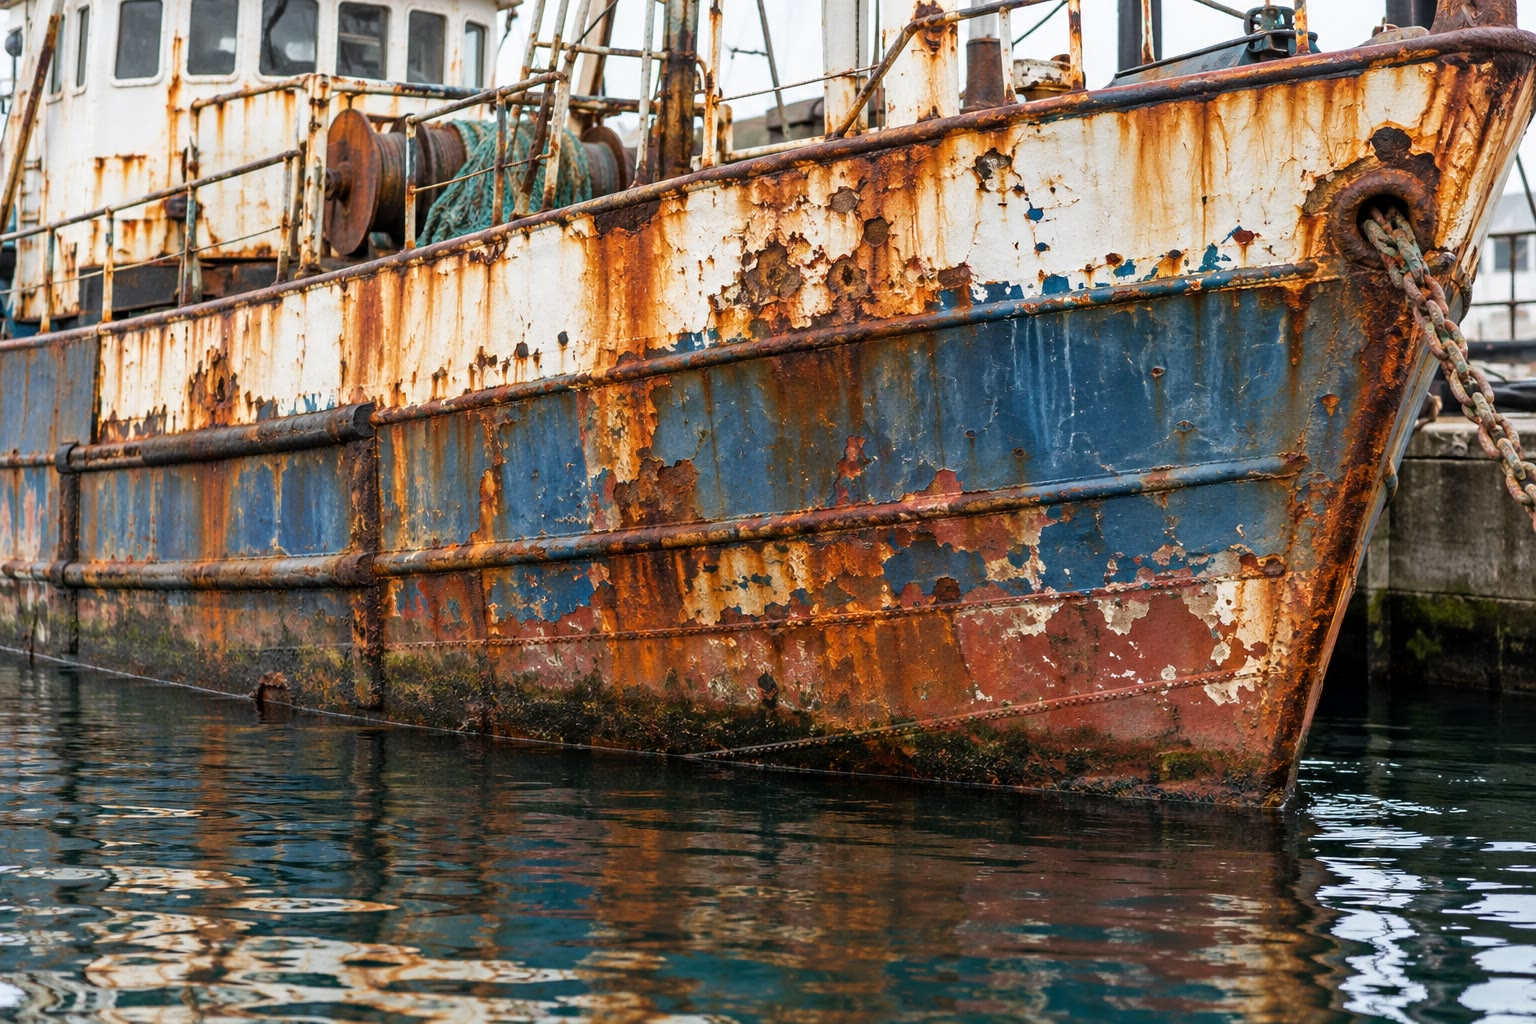
\includegraphics[width=0.55\linewidth]{images/book1/ai/g9-rusty-hull.jpg}

{\small O casco de um barco velho: o aço está enferrujando.}
\end{omfigure}

\section{Os metais no ácido clorídrico}

\begin{inthelab}[Três metais no ácido]
O professor coloca um pedacinho de ferro, um de zinco e um de cobre em
três tubos de ensaio com ácido clorídrico diluído. Sobem bolhas do ferro
e do zinco, devagar no ferro, depressa no zinco, e os metais vão
desaparecendo; com o cobre não acontece nada. O gás, recolhido num tubo
pequeno, dá um estalo agudo: é o hidrogênio. Com o hidróxido de sódio, o
líquido do primeiro tubo dá um \omterm{def:g9:ions:precipitate}{precipitado} verde (\omterm{def:g9:ions:ion}{íons} \ce{Fe^{2+}}), e o
do segundo, um branco (\omterm{def:g9:ions:ion}{íons} \ce{Zn^{2+}}).
\end{inthelab}

\begin{omfigure}
\begin{tikzpicture}[font=\small, scale=1.2]
  \foreach \k/\m/\c/\bub in {0/ferro/black!45/4, 1/zinco/black!25/9, 2/cobre/orange!60!brown/0} {
    \pic[transform shape] at (\k*2.4,0) {testtube={0.55}{omWater!70}};
    \fill[\c] (\k*2.4-0.13,0.08) rectangle (\k*2.4+0.13,0.35);
    \ifnum\bub>0
      \foreach \j in {1,...,\bub} {
        \pgfmathsetmacro\yy{0.45+0.12*\j}
        \pgfmathsetmacro\xx{\k*2.4+0.1*sin(97*\j)}
        \draw[black!55] (\xx,\yy) circle (0.035);
      }
    \fi
    \node[anchor=north, align=center] at (\k*2.4,-0.15) {\m};
  }
  \node[anchor=north, align=center, font=\footnotesize] at (0,-0.6) {bolhas, devagar};
  \node[anchor=north, align=center, font=\footnotesize] at (2.4,-0.6) {bolhas, depressa};
  \node[anchor=north, align=center, font=\footnotesize] at (4.8,-0.6) {nenhuma reação};
\end{tikzpicture}

{\small Ferro, zinco e cobre em ácido clorídrico diluído: o ferro e o
zinco liberam hidrogênio; o cobre não reage.}
\end{omfigure}

\begin{proposition}[Metal mais ácido]\label{prop:g9:metals-acids-corrosion:acid}
Muitos metais --- ferro, zinco, alumínio, magnésio --- reagem com os
\omterm{def:g9:ions:ion}{íons} \ce{H+} de um ácido: o metal desaparece na forma de \omterm{def:g9:ions:ion}{íons} metálicos,
que ficam dissolvidos, e gás hidrogênio é liberado. O cobre, a prata e o
ouro não reagem com o ácido clorídrico.
\end{proposition}

\section{Escrever a equação com íons}

\begin{definition}[Íon espectador]\label{def:g9:metals-acids-corrosion:spectator}
Um \omterm{def:g9:ions:ion}{íon} que está presente numa solução durante uma reação mas não
participa dela, e é encontrado sem mudança no fim, é um \emph{íon
espectador}\index{ion espectador@íon espectador}. Ele é deixado de fora da equação.
\end{definition}

\begin{example}[O ferro e o zinco no ácido clorídrico]\label{ex:g9:metals-acids-corrosion:iron}
O ácido clorídrico contém \omterm{def:g9:ions:ion}{íons} \ce{H+(aq)} e \ce{Cl-(aq)}. Os \omterm{def:g9:ions:ion}{íons}
cloreto são encontrados sem mudança no fim: eles são espectadores. As
equações são
\[
  \ce{Fe(s) + 2H+(aq) -> Fe^{2+}(aq) + H2(g)}, \qquad
  \ce{Zn(s) + 2H+(aq) -> Zn^{2+}(aq) + H2(g)}.
\]
Elas balanceiam ao mesmo tempo os \omterm{def:g7:atoms-and-molecules:atom}{átomos} e as cargas: $+2$ de cada lado.
\end{example}

\begin{method}[Escrever a equação de um metal com um ácido]\label{met:g9:metals-acids-corrosion:write}
\begin{enumerate}
  \item \omterm{def:g7:chemical-reactions:reactant}{Reagentes}: o metal (s) e os \omterm{def:g9:ions:ion}{íons} \ce{H+(aq)}.
  \item Produtos: o \omterm{def:g9:ions:ion}{íon} metálico (aq), com a sua carga habitual, e o
        hidrogênio \ce{H2(g)}.
  \item Balanceie os \omterm{def:g7:atoms-and-molecules:atom}{átomos}, depois verifique que a carga total é a mesma
        dos dois lados.
\end{enumerate}
Para o alumínio: \ce{2Al(s) + 6H+(aq) -> 2Al^{3+}(aq) + 3H2(g)}; carga
$+6$ de cada lado.
\end{method}

\begin{safety}{\ghs[0.8cm]{GHS02}\ghs[0.8cm]{GHS04}}
% ledger: ghs:H2
O hidrogênio liberado é extremamente inflamável. A reação é feita em
tubos de ensaio pequenos, pelo professor, longe de qualquer chama, a não
ser a usada no teste do estalo.
\end{safety}

\section{A corrosão}

\begin{definition}[Corrosão e ferrugem]\label{def:g9:metals-acids-corrosion:corrosion}
A \emph{corrosão}\index{corrosao@corrosão} é o ataque lento de um metal pelas
substâncias à sua volta --- oxigênio, água, ácidos, sais ---, que
transforma o metal em \omterm{def:g9:ions:ion}{íons} ou em compostos como os óxidos. A corrosão do
ferro e do aço produz a \emph{ferrugem}\index{ferrugem}, um óxido de
ferro hidratado, marrom e quebradiço, que se solta em lascas e deixa o
ataque continuar mais fundo.
\end{definition}

\begin{proposition}[Do que o ferro precisa para enferrujar]\label{prop:g9:metals-acids-corrosion:needs}
O ferro só enferruja quando o oxigênio e a água chegam até ele ao mesmo
tempo. O sal dissolvido na água, como nas estradas salgadas no inverno
ou à beira-mar, acelera a \omterm{def:g9:metals-acids-corrosion:corrosion}{ferrugem}.
\end{proposition}

\begin{inthelab}[Três pregos, uma semana]
Três pregos de ferro limpos são colocados em três tubos de ensaio: o
primeiro com \omterm{def:g4:air-a-mixture-of-gases:air}{ar} seco e um agente secante que retira o vapor de água; o
segundo em água fervida para retirar o \omterm{def:g4:air-a-mixture-of-gases:air}{ar} dissolvido, coberta com uma
camada de óleo; o terceiro metade na água da torneira, metade no \omterm{def:g4:air-a-mixture-of-gases:air}{ar}.
Depois de uma semana, só o terceiro prego está enferrujado.
\end{inthelab}

\begin{omfigure}
\begin{tikzpicture}[font=\small, scale=1.2]
  % tube 1: dry air, drying agent
  \pic[transform shape] at (0,0) {testtube={0.18}{white!80!black}};
  \foreach \x/\y in {-0.12/0.15,0.08/0.12,-0.02/0.3,0.12/0.32,-0.14/0.42,0.03/0.48}
    \fill[black!35] (\x,\y) circle (0.05);
  \fill[black!45] (-0.03,1.0) rectangle (0.03,2.4);
  \fill[black!45] (-0.09,2.4) rectangle (0.09,2.48);
  \fill[black!60] (-0.3,2.8) rectangle (0.3,3.1);
  \node[anchor=north, align=center] at (0,-0.15) {ar seco:\\ sem ferrugem};
  % tube 2: boiled water under oil
  \pic[transform shape] at (2.6,0) {testtube={0.7}{omWater!80}};
  \fill[yellow!55!orange!60] (2.36,1.85) rectangle (2.84,2.1);
  \fill[black!45] (2.57,0.3) rectangle (2.63,1.7);
  \fill[black!45] (2.51,1.7) rectangle (2.69,1.78);
  \fill[black!60] (2.3,2.8) rectangle (2.9,3.1);
  \node[anchor=north, align=center] at (2.6,-0.15) {água sem ar:\\ sem ferrugem};
  % tube 3: water and air
  \pic[transform shape] at (5.2,0) {testtube={0.4}{omWater!80}};
  \fill[black!45] (5.17,0.3) rectangle (5.23,2.2);
  \fill[black!45] (5.11,2.2) rectangle (5.29,2.28);
  \fill[orange!60!brown] (5.15,0.9) rectangle (5.25,1.5);
  \node[anchor=north, align=center] at (5.2,-0.15) {água e ar:\\ ferrugem};
  \draw[<-, omProp, thick] (-0.15,0.3) -- (-0.9,0.7) node[left, text=black, font=\footnotesize] {agente secante};
  \draw[<-, omProp, thick] (2.85,1.98) -- (3.6,2.4) node[right, text=black, font=\footnotesize] {óleo};
\end{tikzpicture}

{\small O experimento dos três pregos: o ferro só enferruja onde a água e
o oxigênio chegam juntos até ele, aqui na superfície da água.}
\end{omfigure}

\begin{example}[O alumínio e o cobre se protegem sozinhos]\label{ex:g9:metals-acids-corrosion:protect}
O alumínio é atacado na hora pelo oxigênio do \omterm{def:g4:air-a-mixture-of-gases:air}{ar}, mas a fina camada de
óxido formada gruda no metal e o isola do \omterm{def:g4:air-a-mixture-of-gases:air}{ar}: as esquadrias de alumínio
duram décadas. O cobre, atacado devagar pelo \omterm{def:g4:air-a-mixture-of-gases:air}{ar}, pela água e pelo
dióxido de carbono, fica coberto por uma crosta verde, a pátina, que
também gruda e protege o metal de baixo. Já a \omterm{def:g9:metals-acids-corrosion:corrosion}{ferrugem} se solta em
lascas.
\end{example}

\begin{omfigure}
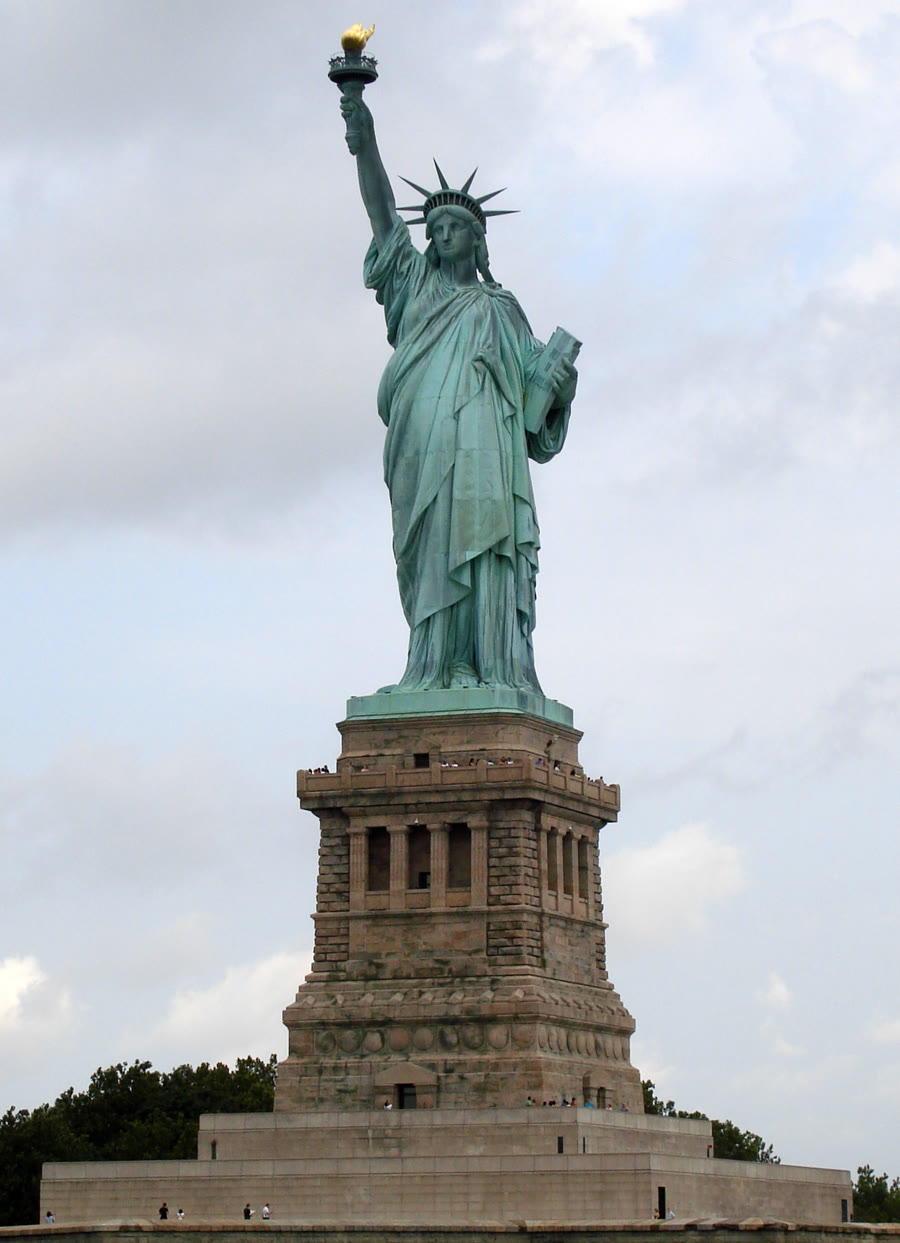
\includegraphics[height=6cm]{images/book1/statue-patina.jpg}

{\small A Estátua da Liberdade: a sua pele de cobre está coberta por uma
pátina verde. Foto: Elcobbola, domínio público.}
\end{omfigure}

\section{Proteger os metais}

\begin{definition}[Galvanização]\label{def:g9:metals-acids-corrosion:galvanising}
A \emph{galvanização}\index{galvanizacao@galvanização} consiste em revestir o aço com
uma camada de zinco, mergulhando-o no zinco derretido. O zinco é atacado
pelo \omterm{def:g4:air-a-mixture-of-gases:air}{ar} e pela água no lugar do aço de baixo: mesmo onde o revestimento
está arranhado, o zinco vizinho sofre a \omterm{def:g9:metals-acids-corrosion:corrosion}{corrosão} primeiro e o aço é
poupado.
\end{definition}

\begin{proposition}[Jeitos de proteger o ferro e o aço]\label{prop:g9:metals-acids-corrosion:ways}
\begin{itemize}
  \item manter a água e o \omterm{def:g4:air-a-mixture-of-gases:air}{ar} longe: tinta, óleo, graxa, um revestimento
        de \omterm{def:g8:plastics:plastic}{plástico};
  \item galvanizar: uma camada de zinco que sofre a \omterm{def:g9:metals-acids-corrosion:corrosion}{corrosão} no lugar do
        aço;
  \item usar aço inoxidável, uma liga de ferro com cromo, que se protege
        sozinha com uma fina camada de óxido isolante;
  \item fixar blocos de zinco nos cascos dos navios: o zinco é corroído
        devagar no lugar do aço, e é substituído de tempos em tempos
        (como isso funciona é explicado num volume universitário).
\end{itemize}
\end{proposition}

\begin{omfigure}
\begin{minipage}[b]{0.52\linewidth}\centering
\begin{tikzpicture}[font=\small]
  \fill[black!35] (0,0) rectangle (5,0.8);
  \fill[black!15] (0,0.8) rectangle (2.2,1.1);
  \fill[black!15] (2.8,0.8) rectangle (5,1.1);
  \fill[omWater!80] (1.6,1.1) rectangle (3.4,1.35);
  \fill[omWater!80] (2.2,0.8) rectangle (2.8,1.1);
  \draw[black!60] (0,0) rectangle (5,0.8);
  \foreach \x in {1.95,2.1} \draw[->, omProp, thick] (\x,1.25) -- (\x+0.05,1.7);
  \node[anchor=west, font=\footnotesize] at (5.1,0.4) {aço};
  \node[anchor=west, font=\footnotesize] at (5.1,0.95) {camada de zinco};
  \node[anchor=south, font=\footnotesize, align=center] at (2.0,1.75) {íons zinco\\ vão para a água};
  \node[anchor=north, font=\footnotesize, align=center] at (2.5,-0.05) {um arranhão: o aço\\ fica exposto, mas o zinco\\ em volta é corroído primeiro};
\end{tikzpicture}

{\small Uma chapa galvanizada arranhada.}
\end{minipage}\hfill
\begin{minipage}[b]{0.44\linewidth}\centering
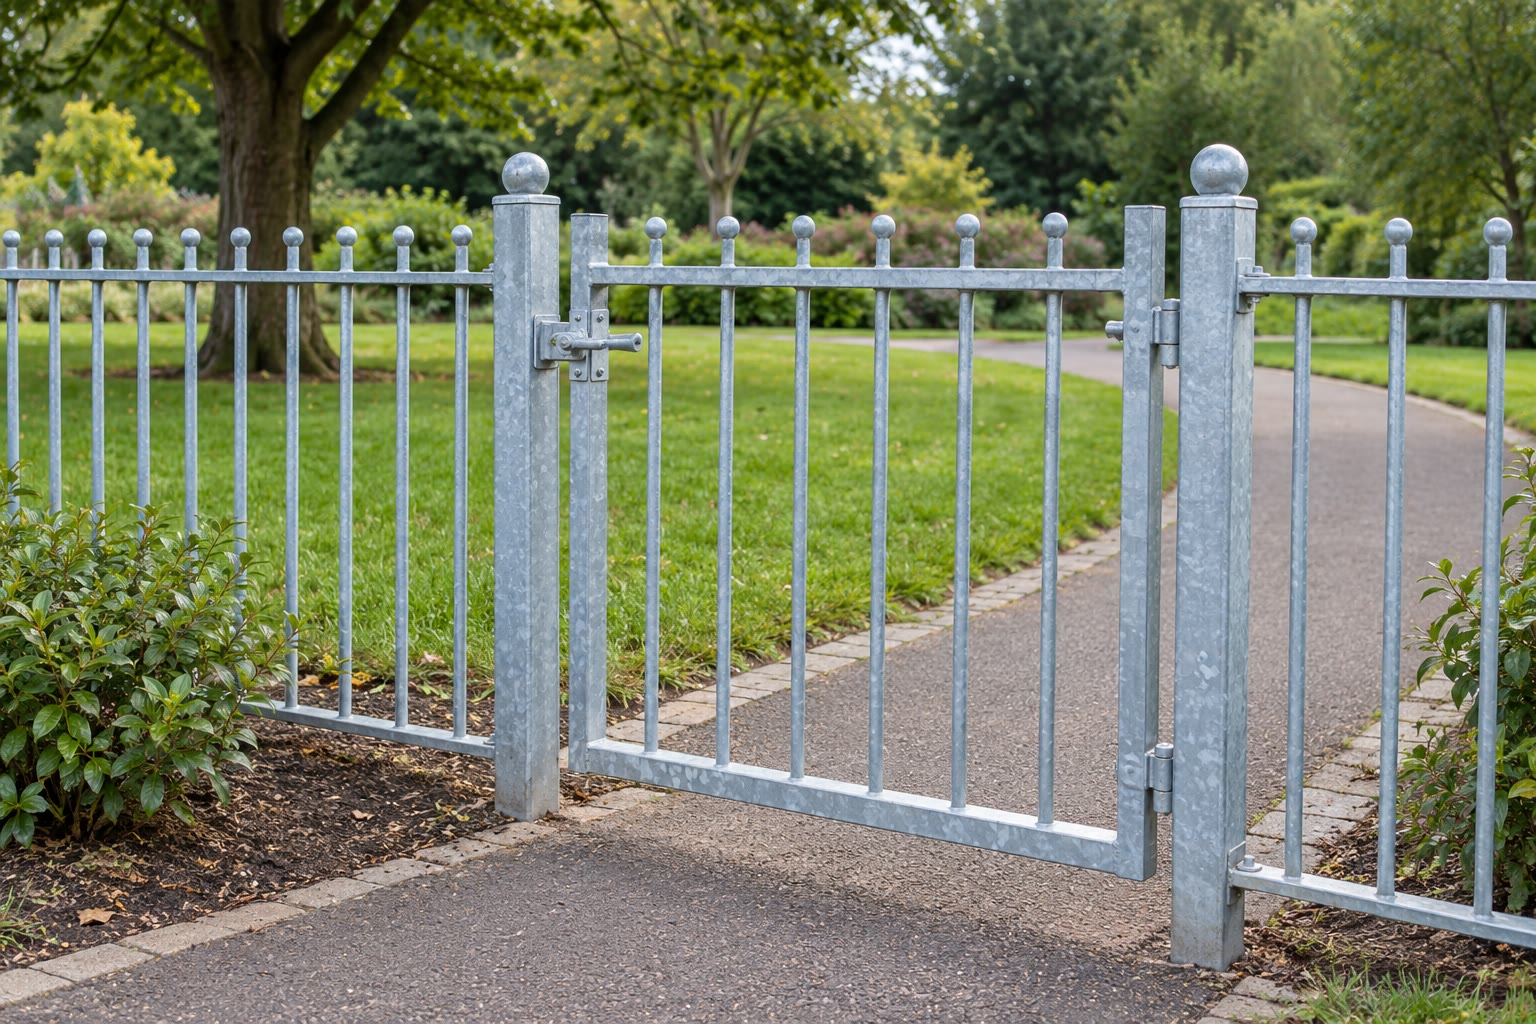
\includegraphics[width=\linewidth,height=4.4cm,keepaspectratio]{images/book1/ai/g9-galvanised-railings.jpg}

{\small Grades de aço galvanizado.}
\end{minipage}
\end{omfigure}

\section{Exercícios}

\begin{exercise}[$\star$]\label{exo:g9:metals-acids-corrosion:1}
Que gás é liberado quando o zinco reage com o ácido clorídrico? Como ele
é identificado?
\end{exercise}

\begin{exercise}[$\star$]\label{exo:g9:metals-acids-corrosion:2}
Quais destes metais reagem com o ácido clorídrico diluído: ferro, cobre,
zinco, ouro, alumínio?
\end{exercise}

\begin{exercise}[$\star$]\label{exo:g9:metals-acids-corrosion:3}
Do que o ferro precisa para enferrujar?
\end{exercise}

\begin{exercise}[$\star$]\label{exo:g9:metals-acids-corrosion:4}
O que é um \omterm{def:g9:metals-acids-corrosion:spectator}{íon espectador}? Dê o nome do \omterm{def:g9:metals-acids-corrosion:spectator}{íon espectador} quando o ferro
reage com o ácido clorídrico.
\end{exercise}

\begin{exercise}[$\star\star$]\label{exo:g9:metals-acids-corrosion:5}
Escreva a equação da reação do magnésio com os \omterm{def:g9:ions:ion}{íons} \ce{H+} de um ácido
(o \omterm{def:g9:ions:ion}{íon} magnésio é \ce{Mg^{2+}}). Verifique as cargas.
\end{exercise}

\begin{exercise}[$\star\star$]\label{exo:g9:metals-acids-corrosion:6}
Depois que o ferro reagiu com o ácido clorídrico, como você pode mostrar
que a solução contém \omterm{def:g9:ions:ion}{íons} ferro(II)?
\end{exercise}

\begin{exercise}[$\star\star$]\label{exo:g9:metals-acids-corrosion:7}
Olhe a figura dos três pregos. Por que a água do segundo tubo é fervida
e coberta com óleo?
\end{exercise}

\begin{exercise}[$\star\star$]\label{exo:g9:metals-acids-corrosion:8}
Por que um carro enferruja mais depressa numa cidade onde as ruas são
salgadas no inverno?
\end{exercise}

\begin{exercise}[$\star\star$]\label{exo:g9:metals-acids-corrosion:9}
Por que as esquadrias de alumínio não são destruídas pela \omterm{def:g9:metals-acids-corrosion:corrosion}{corrosão},
embora o alumínio reaja com o oxigênio do \omterm{def:g4:air-a-mixture-of-gases:air}{ar}?
\end{exercise}

\begin{exercise}[$\star\star$]\label{exo:g9:metals-acids-corrosion:10}
Dê três jeitos de proteger da \omterm{def:g9:metals-acids-corrosion:corrosion}{ferrugem} o quadro de aço de uma bicicleta.
\end{exercise}

\begin{exercise}[$\star\star\star$]\label{exo:g9:metals-acids-corrosion:11}
Escreva e verifique a equação da reação do alumínio com os \omterm{def:g9:ions:ion}{íons} \ce{H+}
de um ácido. Quantas \omterm{def:g7:atoms-and-molecules:molecule}{moléculas} de hidrogênio são formadas para 200
\omterm{def:g7:atoms-and-molecules:atom}{átomos} de alumínio?
\end{exercise}

\begin{exercise}[$\star\star\star$]\label{exo:g9:metals-acids-corrosion:12}
Um balde de aço galvanizado é arranhado até o aço. Explique por que o aço
no fundo do arranhão não enferruja durante muito tempo.
\end{exercise}

\section{Problema: qual é a espessura do zinco?}

\begin{problem}[{Problema de fim de semana --- dissolver o revestimento
de zinco de uma chapa galvanizada para descobrir a espessura dele}]
\label{pb:g9:metals-acids-corrosion:1}
% ledger: rho:Zn
Uma chapa de aço galvanizado, um quadrado de \qty{10.0}{cm} de lado, é
revestida de zinco nas duas faces (as bordas são desprezadas). Num
laboratório, o professor a pesa, \qty{125.6}{g}, e depois a mergulha em
ácido clorídrico com um aditivo que impede o ácido de atacar o aço.
Quando o borbulhamento para, a chapa é enxaguada, secada e pesada de
novo: \qty{113.5}{g}. A massa de \qty{1}{cm^3} de zinco é \qty{7.13}{g}.

\medskip
\noindent\textbf{Parte I --- A reação.}
\begin{enumerate}
  \item Escreva a equação da reação do zinco com os \omterm{def:g9:ions:ion}{íons} \ce{H+} do
        ácido.
  \item Que gás provoca o borbulhamento? Descreva o teste dele.
  \item Que teste mostraria, depois, os \omterm{def:g9:ions:ion}{íons} zinco na solução?
  \item Dê o nome dos \omterm{def:g9:metals-acids-corrosion:spectator}{íons espectadores}.
\end{enumerate}

\medskip
\noindent\textbf{Parte II --- O zinco.}
\begin{enumerate}[resume]
  \item Que massa de zinco se dissolveu?
  \item Por que o borbulhamento é um sinal de que o zinco ainda não se
        dissolveu todo?
  \item O que aconteceria com o aço se o ácido não tivesse o aditivo? Que
        teste mostraria isso?
  \item Por que o zinco protege o aço da chapa enquanto ele estiver lá?
\end{enumerate}

\medskip
\noindent\textbf{Parte III --- A espessura.}
\begin{enumerate}[resume]
  \item Qual é a área total revestida da chapa, em \unit{cm^2}?
  \item Que volume o zinco ocupava?
  \item Deduza a espessura da camada de zinco, em centímetros.
  \item Expresse essa espessura em micrômetros
        (\qty{1}{cm} $= \qty{10000}{\micro m}$).
\end{enumerate}
\end{problem}
